\documentclass[11pt,a4paper]{article}

\usepackage[T1]{fontenc}
\usepackage[utf8]{inputenc}
\usepackage{lmodern}
\usepackage[margin=24mm]{geometry}
\usepackage{amsmath,amssymb}
\usepackage{booktabs,array,tabularx}
\usepackage{graphicx}
\usepackage[section]{placeins}
\usepackage{microtype}
\usepackage{enumitem}
\usepackage{xurl}
\usepackage[hidelinks]{hyperref}
\usepackage{bookmark}

\setlength{\emergencystretch}{2em}
\setlist{itemsep=0.35em,topsep=0.5em}
\urlstyle{tt}
\numberwithin{equation}{section}
\newcommand{\units}[1]{\,\mathrm{#1}}
\newcommand{\mat}[1]{\mathsf{#1}}

\title{A synthetic DBA ring for KV tune-shift benchmarks\\
and AI-assisted lattice design}
\author{A Adelmann \& Hugo}
\date{1 November 2026}
\hypersetup{pdftitle={A synthetic DBA ring for KV tune-shift benchmarks and AI-assisted lattice design}}

\begin{document}
\maketitle

\begin{abstract}
A six-cell synthetic ring provides a common model for two tasks: comparison
of space-charge tune shifts with the OPALX FFT2D5 solver, and evaluation of
AI-assisted lattice reconstruction and optimization. A quadratic
six-dimensional Hamiltonian specifies the external linear optics, including
dispersion and longitudinal transport. A matched coasting
Kapchinskij--Vladimirskij (KV) distribution supplies analytic transverse
self-fields; numerical envelope matching and phase integration determine
the incoherent tunes as functions of current and charge. This note defines
the canonical conventions, cell parameters, benchmark operating points,
and validation procedure. The machine-design task first reconstructs the
ring from its cell and then adjusts the cell to prescribed tune targets.
The reference calculations do not constitute an end-to-end validation of
FFT2D5 tracking.
\end{abstract}

\section{Purpose and model scope}
\label{sec:scope}

The ring uses six identical cells, each containing two sector bends, two
drifts, and one quadrupole. Its double-bend cell geometry motivates the
DBA label, but the selected lattice is deliberately non-achromatic. The
same geometry and focusing coefficients define both the space-charge
benchmark and the machine-design task.

The external model assumes hard-edge fields, paraxial motion,
first-order momentum deviations, and a fixed reference energy. It
excludes fringe fields, chromatic nonlinearities, radio-frequency (RF)
fields, radiation, and errors. The Hamiltonian is complete within this
quadratic model; it does not describe exact nonlinear motion in magnetic
fields. The KV comparison further assumes zero momentum spread, a
longitudinally uniform coasting beam, and locally straight transverse
space-charge forces.

Section~\ref{sec:hamiltonian} defines the external Hamiltonian and cell.
Section~\ref{sec:kv} specifies the KV reference, and
Section~\ref{sec:fft2d5} describes the comparison with FFT2D5, the OPALX
2.5-dimensional space-charge solver. Section~\ref{sec:design} defines the
reconstruction and optimization tasks. File paths are relative to the
project root, one directory above \path{TeX/}.

\section{External Hamiltonian and ring construction}
\label{sec:hamiltonian}

\subsection{Canonical coordinates}

The independent variable is the reference arc length $s$, measured in
metres. A prime denotes differentiation with respect to $s$. The canonical
state comprises three conjugate pairs,
\begin{equation}
  \mathbf u=(x,p_x,y,p_y,\zeta,\eta)^{\mat T}.
  \label{eq:state}
\end{equation}
The transverse coordinates $x$ and $y$ are measured in metres, and the
normalized canonical momenta are
\begin{equation}
  p_x=\frac{P_x}{p_0},\qquad p_y=\frac{P_y}{p_0},
  \label{eq:momentum}
\end{equation}
where $p_0$ is the reference momentum. The ideal-magnet gauge used here
has zero transverse vector potential. To linear order, $p_x$ and $p_y$
therefore equal the transverse slopes.

The longitudinal pair records arrival time and energy deviation:
\begin{equation}
  \zeta=\beta_0c\left(\frac{s}{\beta_0c}-t\right),\qquad
  \eta=\frac{E-E_0}{\beta_0^2E_0}.
  \label{eq:longitudinal}
\end{equation}
Here $t$ is the arrival time, $E_0$ is the reference total energy, and
$\beta_0$ and $\gamma_0$ are the reference relativistic factors for
$2.5\units{MeV}$ protons. The coordinate $\zeta$ has units of metres and
is positive for early arrival; $\eta$ is dimensionless and equals the
relative momentum deviation $\Delta p/p_0$ only to first order.

OPALX normalizes particle momentum by $mc$ rather than $p_0$. For an
on-momentum proton, the corresponding transverse conversion is
\begin{equation}
  \frac{P_x}{mc}=\beta_0\gamma_0p_x,
  \label{eq:opalx-momentum}
\end{equation}
with the analogous expression in the vertical plane.

The local horizontal coordinate points outward in a bend, and the local
vertical coordinate points along $y$. At the ring entrance, positive
curvature $h$ bends the reference trajectory towards negative laboratory
$X$. In the laboratory $(X,Z)$ plane, the tangent and orientation satisfy
\begin{equation}
  \hat{\mathbf t}=(\sin\theta,\cos\theta),\qquad \theta'=-h.
  \label{eq:geometry}
\end{equation}
The entry and exit placements in \path{model/machine.json} follow this
convention and match the copied baseline input deck.

\subsection{Hamiltonian and exact linear maps}

With these conventions, the scaled, dimensionless external Hamiltonian is
\begin{equation}
  H_{\mathrm{ext}}(\mathbf u;s)
  =\frac{p_x^2+p_y^2}{2}
   +\frac{k_x(s)x^2+k_y(s)y^2}{2}
   -h(s)x\eta+\frac{\eta^2}{2\gamma_0^2}.
  \label{eq:external-hamiltonian}
\end{equation}
The curvature $h$ has units of $\mathrm{m^{-1}}$, and the focusing
coefficients $k_x$ and $k_y$ have units of $\mathrm{m^{-2}}$. Hamilton's
equations give
\begin{equation}
  \begin{aligned}
    x'&=p_x,                 & p_x'&=-k_xx+h\eta,\\
    y'&=p_y,                 & p_y'&=-k_yy,\\
    \zeta'&=-hx+\eta/\gamma_0^2, & \eta'&=0.
  \end{aligned}
  \label{eq:hamilton-equations}
\end{equation}
The coefficients are constant within each element. The coordinates and
canonical momenta remain continuous at hard edges; the model applies no
thin-edge kicks. Each element conserves its autonomous Hamiltonian,
whereas the explicitly $s$-dependent Hamiltonian of the complete ring is
not a globally conserved scalar.

Let $\mat G$ denote the Hessian of $H_{\mathrm{ext}}$ with respect to
$\mathbf u$, and let
\begin{equation}
  \mat J=\operatorname{diag}(\mat J_2,\mat J_2,\mat J_2),\qquad
  \mat J_2=\begin{pmatrix}0&1\\-1&0\end{pmatrix}.
  \label{eq:symplectic-form}
\end{equation}
The linear equations and exact map for an element of length $L$ are
\begin{equation}
  \mathbf u'=\mat J\mat G\mathbf u,\qquad
  \mat M(L)=\exp(L\mat J\mat G).
  \label{eq:element-map}
\end{equation}
These maps are symplectic and include dispersion and longitudinal
coupling. In beam order, the cell and ring maps are
\begin{equation}
  \mat M_{\mathrm{cell}}
    =\mat M_{B2}\mat M_{D2}\mat M_Q\mat M_{D1}\mat M_{B1},\qquad
  \mat M_{\mathrm{ring}}=\mat M_{\mathrm{cell}}^6.
  \label{eq:ring-map}
\end{equation}
The canonical Hamiltonian context is described in Ref.~\cite{tracking};
the coordinate conventions and signs of the present quadratic model are
specified explicitly in Eqs.~\eqref{eq:state}--\eqref{eq:ring-map} and
checked against closed-form sector-bend maps.

\subsection{Cell parameters and zero-current optics}

Table~\ref{tab:cell} specifies the ordered cell. Repeating it six times
produces 30 elements, including twelve $30^\circ$ sector bends of radius
$2\units{m}$. The total bend angle is $2\pi$, and the circumference is
$25.76637061436\units{m}$.
Figure~\ref{fig:ring-lattice} shows the reference geometry and element
sequence in laboratory coordinates.

\begin{table}[htbp]
  \centering
  \caption{Hard-edge cell parameters. The coefficients $k_x$ and $k_y$
  describe physical focusing in Eq.~\eqref{eq:external-hamiltonian}; they
  are not OPALX input attributes. Elements appear in beam order.}
  \label{tab:cell}
  \begin{tabular}{lrrrr}
    \toprule
    Element & $L$ [m] & $h$ [$\mathrm{m^{-1}}$]
      & $k_x$ [$\mathrm{m^{-2}}$] & $k_y$ [$\mathrm{m^{-2}}$]\\
    \midrule
    $B1$ & $\pi/3$ & $0.5$ & $0.25$ & $0$\\
    $D1$ & $1$ & $0$ & $0$ & $0$\\
    $Q$  & $0.2$ & $0$ & $-2.84$ & $+2.84$\\
    $D2$ & $1$ & $0$ & $0$ & $0$\\
    $B2$ & $\pi/3$ & $0.5$ & $0.25$ & $0$\\
    \bottomrule
  \end{tabular}
\end{table}

\begin{figure}[htbp]
  \centering
  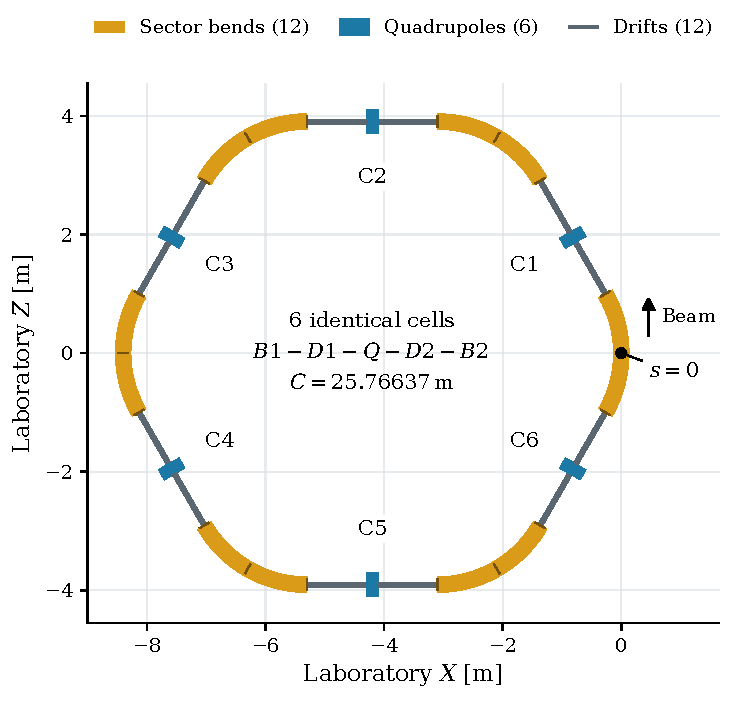
\includegraphics[width=0.88\linewidth]{figures/ring-lattice.pdf}
  \caption{Reference geometry of the six-cell synthetic ring for the
  $2.5\units{MeV}$ proton benchmark. Each cell follows the sequence
  $B1$--$D1$--$Q$--$D2$--$B2$; the complete ring contains twelve
  sector bends, twelve drifts, and six quadrupoles. The laboratory
  coordinates have equal scale. The arrow indicates the initial beam
  direction at $s=0$, and short transverse strokes distinguish adjacent
  bends. Magnet widths are schematic and do not represent apertures.}
  \label{fig:ring-lattice}
\end{figure}

The proton OPALX input uses $K_1=-2.84\units{m^{-2}}$ to implement the
quadrupole coefficients in Table~\ref{tab:cell}. The historical electron
benchmark uses the opposite sign. Interpreting the OPALX attribute
$K_1$ therefore requires the particle and charge convention.

The full positive zero-current tunes are
\begin{equation}
  Q_x(0)=0.770107569133,\qquad Q_y(0)=1.689536397020.
  \label{eq:bare-tunes}
\end{equation}
The principal fractional one-turn eigenphases quoted in the original
benchmark, $0.229892431$ and $0.310463603$, are compatible with these
tunes but do not specify their full positive values. The generator selects
a cell phase in $(0,2\pi)$ from the sign of the corresponding transverse
map entry $M_{12}$ and multiplies the phase by six. An independent KV
phase integral verifies this branch at the baseline. Local optimization
remains near that branch; a design with more than one oscillation per
cell requires independent phase unwrapping along $s$.

The periodic horizontal dispersion at the entrance is approximately
$9.337460094\units{m}$, with zero slope. The longitudinal motion drifts;
the machine provides no longitudinal confinement.

\section{Matched coasting KV reference}
\label{sec:kv}

\subsection{Envelope conventions and matching}

The KV reference uses zero momentum spread, $\eta=0$, and a
longitudinally uniform coasting beam. An initially uniform coasting beam
remains longitudinally uniform in this ideal model. The transverse edge
radii $a$ and $b$, measured in metres, relate to the root-mean-square
(rms) beam sizes through
\begin{equation}
  a=2\sigma_x,\qquad b=2\sigma_y.
  \label{eq:edge-radii}
\end{equation}
The geometric edge emittances $\mathcal E_x$ and $\mathcal E_y$
(\texttt{Ex} and \texttt{Ey} in the original model notation) are four times the corresponding geometric rms emittances. The baseline rms
emittance in each plane is $3\times10^{-6}\units{m\,rad}$.

For positive proton current $I$, the Alfv\'en current and generalized
perveance are
\begin{equation}
  I_A=\frac{4\pi\epsilon_0m_pc^3}{e},\qquad
  K=\frac{2I}{I_A\beta_0^3\gamma_0^3},
  \label{eq:perveance}
\end{equation}
where $m_p$ is the proton mass, $e$ is the elementary charge, and
$\epsilon_0$ is the vacuum permittivity. The coupled KV envelope
equations are
\begin{equation}
  \begin{aligned}
    a''+k_xa-\frac{\mathcal E_x^2}{a^3}-\frac{2K}{a+b}&=0,\\
    b''+k_yb-\frac{\mathcal E_y^2}{b^3}-\frac{2K}{a+b}&=0.
  \end{aligned}
  \label{eq:envelopes}
\end{equation}
Reference~\cite{prior} describes the KV envelope and perveance
conventions. The calculation rematches the periodic envelopes at each
current while holding the external focusing fixed. The self-field is
analytic; envelope matching and phase integration are numerical.

\subsection{Collective potential and particle tunes}

Inside the uniform KV ellipse, the transverse collective contribution to
the test-particle Hamiltonian is
\begin{equation}
  H_{\mathrm{sc}}
  =-\frac{K}{a+b}\left(\frac{x^2}{a}+\frac{y^2}{b}\right).
  \label{eq:sc-hamiltonian}
\end{equation}
The resulting effective focusing coefficients are
\begin{equation}
  k_{x,\mathrm{eff}}=k_x-\frac{2K}{a(a+b)},\qquad
  k_{y,\mathrm{eff}}=k_y-\frac{2K}{b(a+b)}.
  \label{eq:effective-focusing}
\end{equation}
Equation~\eqref{eq:sc-hamiltonian} describes an interior mean-field
potential with self-consistently matched envelopes. Its quadratic form
does not apply outside the ellipse. The model neither sums
finite-particle pair interactions nor includes six-dimensional collective
dynamics with longitudinal space charge. Self-consistency enters through
Eq.~\eqref{eq:envelopes}; retaining the zero-current beam sizes as the
current increases would change the model. Additive functions of $s$ do
not affect the transverse motion.

The KV distribution forms a uniform shell in normalized four-dimensional
transverse phase space, with invariant
\begin{equation}
  \left(\frac{x}{a}\right)^2
  +\left(\frac{ap_x-a'x}{\mathcal E_x}\right)^2
  +\left(\frac{y}{b}\right)^2
  +\left(\frac{bp_y-b'y}{\mathcal E_y}\right)^2=1.
  \label{eq:kv-invariant}
\end{equation}
A filled four-dimensional ball represents a different distribution. The
full positive incoherent particle tunes follow from the matched envelopes:
\begin{equation}
  Q_x(I)=\frac{6}{2\pi}\int_{\mathrm{cell}}
             \frac{\mathcal E_x}{a(s)^2}\,\mathrm ds,\qquad
  Q_y(I)=\frac{6}{2\pi}\int_{\mathrm{cell}}
             \frac{\mathcal E_y}{b(s)^2}\,\mathrm ds.
  \label{eq:kv-tunes}
\end{equation}
These tunes describe individual-particle motion rather than centroid
motion or envelope modes. Finite amplitudes and curvature in an OPALX
field tracker can produce departures from the paraxial, locally straight
space-charge reference. Mesh and timestep convergence alone do not remove
such model differences.

\section{Comparison with FFT2D5}
\label{sec:fft2d5}

\subsection{Charge normalization and field reference}

A controlled comparison uses the beam parameters of
Section~\ref{sec:kv}, open transverse boundaries, and no RF fields or
pipe-image forces. FFT2D5 uses laboratory-frame line charge and open
transverse slice solves. Its longitudinal-field mode must be
\path{FFT2D5LongitudinalFieldMode::None} for the purely transverse
comparison; the input-deck spelling must be checked when constructing
the run.

The current fixes the line charge $\lambda$, which in turn fixes the
charge represented by a full ring or a finite segment:
\begin{equation}
  \begin{aligned}
    \lambda&=\frac{I}{\beta_0c}, &
    N_{\mathrm{ring}}&=\frac{\lambda C}{e},\\
    Q_{\mathrm{ring}}&=\lambda C, &
    Q_{\mathrm{segment}}&=\lambda L_{\mathrm{segment}},\\
    q_{\mathrm{macro}}&=\frac{Q_{\mathrm{segment}}}{N_{\mathrm{macro}}}.
  \end{aligned}
  \label{eq:charge}
\end{equation}
Here $C$ is the circumference, $L_{\mathrm{segment}}$ is the represented
segment length, and $N_{\mathrm{macro}}$ is the number of macroparticles
in that segment. The line charge has units of coulombs per metre.

A full coasting ring requires particles distributed around the closed
path with the appropriate local matched covariance at each $s$. A finite
segment requires uniform interior slices and suitable longitudinal
handling. The zero-length observation section in \path{kv-section.txt}
cannot represent a charged coasting beam, and an isolated bunch with open
boundaries describes a different physical model. Full-ring longitudinal
wrapping and continuity across the path seam require verification before
a ring comparison can be claimed.

Within the KV ellipse, the analytic laboratory electric field and the
associated magnetic field are
\begin{equation}
  \begin{aligned}
    E_x&=\frac{\lambda x}{\pi\epsilon_0a(a+b)},&
    E_y&=\frac{\lambda y}{\pi\epsilon_0b(a+b)},\\
    \mathbf B&=\frac{\beta_0}{c}\,\hat{\mathbf t}\times\mathbf E.
  \end{aligned}
  \label{eq:fields}
\end{equation}
The magnetic field reduces the net transverse force to
\begin{equation}
  \mathbf F_\perp=\frac{e\mathbf E_\perp}{\gamma_0^2}.
  \label{eq:force}
\end{equation}
The electric field in Eq.~\eqref{eq:fields} already uses laboratory
normalization and requires no additional factor of $\gamma_0$. Combining
the field and force expressions gives
\begin{equation}
  \frac{e(E_x/x)}{p_0\beta_0c\gamma_0^2}
     =\frac{2K}{a(a+b)},
  \label{eq:force-gradient}
\end{equation}
which connects a local field-gradient check to the defocusing term in
Eq.~\eqref{eq:effective-focusing}.

\subsection{Reference operating points}

Table~\ref{tab:operating-points} lists the reference currents and tunes.
The tune shifts are defined by $\Delta Q_x=Q_x(I)-Q_x(0)$ and
$\Delta Q_y=Q_y(I)-Q_y(0)$. The principal comparison point has
$I=10.399311\units{mA}$ and $\Delta Q_y=-0.2$.

\begin{table}[htbp]
  \centering
  \caption{Coasting KV reference for $2.5\units{MeV}$ protons with
  geometric rms emittances of $3\times10^{-6}\units{m\,rad}$ in each
  plane. The full positive tunes $Q_x$ and $Q_y$ follow from the
  numerically matched periodic envelopes. The final row is
  envelope-unstable and serves only as a stress case.}
  \label{tab:operating-points}
  \small
  \setlength{\tabcolsep}{5pt}
  \begin{tabularx}{\linewidth}{rrrrr>{\raggedright\arraybackslash}X}
    \toprule
    $I$ [mA] & $Q_x$ & $Q_y$ & $\Delta Q_x$ & $\Delta Q_y$ & Role\\
    \midrule
    $0$ & $0.770108$ & $1.689536$ & $0$ & $0$ & Bare optics\\
    $4.748770$ & $0.623940$ & $1.589536$ & $-0.146167$ & $-0.1$
      & First collective comparison\\
    $10.399311$ & $0.484005$ & $1.489536$ & $-0.286102$ & $-0.2$
      & Principal comparison\\
    $17.402677$ & $0.359252$ & $1.389536$ & $-0.410855$ & $-0.3$
      & Envelope-unstable stress case\\
    \bottomrule
  \end{tabularx}
\end{table}

At the principal comparison point, the total ring charge is
$12.26826245\units{nC}$, corresponding to
$7.65724714\times10^{10}$ protons. The entrance rms beam sizes are
$\sigma_x=6.042810\units{mm}$ and $\sigma_y=2.480302\units{mm}$.
At the highest current in Table~\ref{tab:operating-points}, the envelope
multiplier is approximately $1.069761$ per cell. That periodic solution
is therefore unsuitable as a stable matched-beam reference.

Figure~\ref{fig:kv-tune-shift-charge} expresses the analytic reference
as a function of total coasting ring charge. The charge normalization is
that of Eq.~\eqref{eq:charge}; it is not the charge of an arbitrary
finite simulation segment. Crosses identify sampled periodic solutions
with envelope instability. The scan brackets the onset of this
instability between $15.740\units{nC}$ and $16.424\units{nC}$; it does
not locate an exact threshold.

\begin{figure}[htbp]
  \centering
  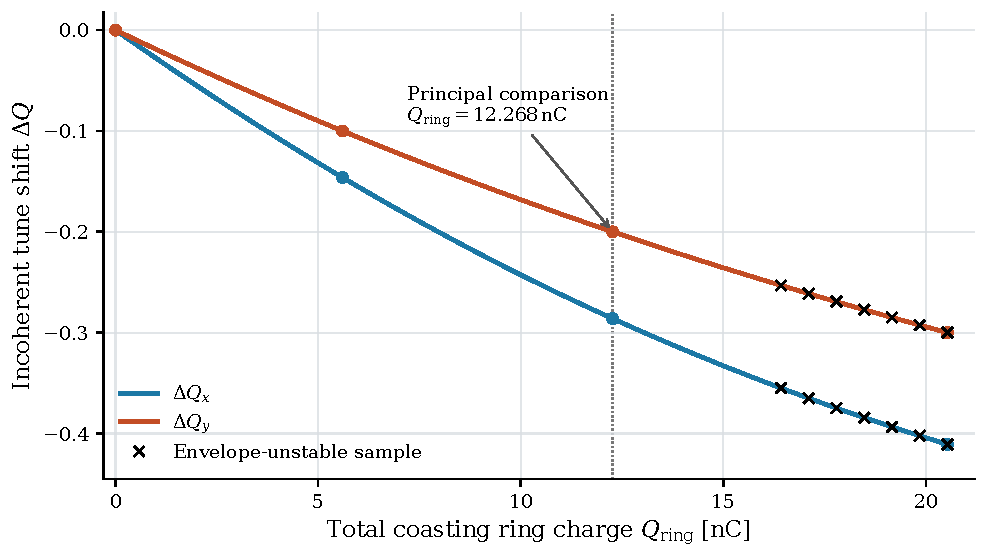
\includegraphics[width=0.96\linewidth]{figures/kv-tune-shift-charge.pdf}
  \caption{Incoherent KV tune shifts versus total coasting ring charge
  for the baseline $2.5\units{MeV}$ proton lattice, with geometric rms
  emittances of $3\times10^{-6}\units{m\,rad}$ in both planes and zero
  momentum spread. The curves join the saved periodic-envelope
  solutions for $\Delta Q_x$ and $\Delta Q_y$; circles mark the
  operating points in Table~\ref{tab:operating-points}, and crosses mark
  envelope-unstable samples. The dotted line identifies the principal
  comparison point, $Q_{\mathrm{ring}}=12.268\units{nC}$, where
  $\Delta Q_y=-0.2$. The self-fields are analytic, while envelope
  matching and phase integration are numerical. These curves are
  independent references, not FFT2D5 tracking results.}
  \label{fig:kv-tune-shift-charge}
\end{figure}

\subsection{Solver validation procedure}

The independent reference is available, but end-to-end OPALX FFT2D5
tracking remains to be validated. The comparison should proceed through
the following stages:
\begin{enumerate}[label=(\roman*)]
  \item Establish convergence of the bare-ring particle and reference
  orbits and of the zero-charge tunes in OPALX. Historical tracking
  reports refer to earlier source revisions and do not establish the
  behavior of the current implementation.
  \item Compare the FFT2D5 interior field gradients and net transverse
  force at a fixed matched section with Eqs.~\eqref{eq:fields}--\eqref{eq:force-gradient}.
  Check deposited charge and line density as well as the fields, then
  repeat the comparison at a curved section to expose coordinate and
  reference-path errors.
  \item Transport the correctly normalized matched source through one
  cell. Compare envelopes and projected moments with the reference at
  every element boundary.
  \item Track the stable coasting operating points over many turns.
  Measure individual-particle tunes at a consistent observation plane,
  with the tune branches unfolded. Centroid motion or a principal
  fast-Fourier-transform peak alone does not provide this comparison.
  Include a zero-charge run with the same numerical settings.
  \item Quantify sensitivity to timestep, transverse mesh spacing and
  domain size, longitudinal slice spacing, macroparticle count, and
  spectral observation length. Hold the physical parameters fixed and
  report absolute tune errors and errors in $\Delta Q$. Set acceptance tolerances
  from the convergence evidence.
\end{enumerate}
Parameter studies use one Message Passing Interface (MPI) rank. Dedicated
single-rank and multi-rank consistency checks belong to solver validation,
rather than to the serial reference calculation. No OPALX or MPI solver
validation has yet been completed for this standalone package.

\section{AI-assisted reconstruction and optimization}
\label{sec:design}

\subsection{Reconstruction task}

The reconstruction task supplies an AI system with
\path{model/cell.json} and the Hamiltonian specification in
Section~\ref{sec:hamiltonian}. The evaluator retains
\path{model/machine.json} as the reference output when an independent
reconstruction is required.

The system must derive the six Hamilton equations, construct the exact
map of each element, compose the ordered cell map, and repeat the cell
six times. It must also integrate the reference geometry and report all
30 placements, the cell and ring maps, circumference, total bend angle,
periodic dispersion, full tunes, and symplectic residuals. The proton
sign convention applies throughout. At zero current, the reconstructed
tunes must reproduce the independent envelope phase integrals; principal
one-turn eigenphases alone do not determine the full tune branches.

The baseline evaluator is \path{model/machine.py}, and the checks are
implemented in \path{tests/test_machine.py}. The reconstruction targets
are the circumference and cell geometry of Section~\ref{sec:hamiltonian},
the full tunes in Eq.~\eqref{eq:bare-tunes}, and the entrance dispersion
of $9.337460094\units{m}$ with zero slope. The tests use near-roundoff
tolerances for exact maps and geometry, and $2\times10^{-10}$ for the
comparison with numerically integrated envelope phases. These are
model-verification tolerances, not acceptance criteria for
particle-in-cell (PIC) tracking. The reconstruction must state the
scope of the quadratic model separately from that of exact nonlinear
field tracking.

\subsection{Local tune optimization}

After reconstruction, the design task adjusts the cell to illustrative
full tune targets $(Q_x,Q_y)=(0.8,1.7)$. These values define a
demonstration rather than a proposed operating point or an optimal
physics choice. The two free parameters are the physical quadrupole
coefficient and the common length of the two drifts. The particle,
reference energy, bend radii and angles, quadrupole length, and cell
count remain fixed.

A candidate must have positive lengths, transversely stable cell
optics, symplectic maps, and closed reference geometry. The circumference
may change. Fixing it would generally prevent these two parameters from
matching two arbitrary tune targets; the design would then require an
additional justified degree of freedom or a revised objective.

For each candidate, the system must export the cell specification, the
complete machine, and a KV configuration with exactly the same element
coefficients. It must then rematch the KV beam and recompute the
charge-dependent tune shifts. Envelope-unstable solutions cannot serve
as stable comparison points. Matching the bare tunes alone does not
establish collective stability or robustness.

The script \path{model/optimize.py} provides a deterministic local
reference optimizer for evaluating proposed designs. It does not
demonstrate independent AI design and does not search globally across
tune branches. It reports failure when local matching encounters an
unstable or nonphysical cell, or when the calculation fails to converge.

The worked example in \path{designs/demo-qx0.8-qy1.7/} contains a
complete machine with full tunes $(0.8,1.7)$ and a compatible
\path{kv-config.json} for the analytic scan. Evaluation should consider
the achieved optics, geometry, collective stability, reproducibility,
and stated design tradeoffs.

\section{Reference implementation and validation status}
\label{sec:implementation}

The script \path{tune-shift-ring/analysis/run_model.py} regenerates the
current scan, charge normalization, matched periodic envelopes, particle
tunes, envelope-stability diagnostics, and local electric-field
gradients. Each run writes its comparison targets to
\path{fft2d5_reference.json} in a new result directory. These outputs
provide the independent reference for the staged solver comparison of
Section~\ref{sec:fft2d5}; they do not establish FFT2D5 tracking accuracy.

The machine representation and the matched KV calculation serve
complementary purposes. The former specifies the external linear
machine for reconstruction and design; the latter supplies the
collective reference against which a numerical space-charge solver can
be tested. Both retain the model assumptions and limits stated in
Section~\ref{sec:scope}.

The script \path{TeX/make_figures.py} regenerates the lattice and
tune-shift figures from \path{model/machine.json} and the baseline scan
selected by \path{REFERENCE_RUNS.json}. It verifies the charge
normalization and geometry and records input hashes in
\path{TeX/figures/provenance.json}. The vector PDF figures and PNG
previews are stored in \path{TeX/figures/}.

\begin{thebibliography}{9}
\bibitem{prior}
C.~Prior, \emph{Modelling with Space-Charge}, CERN Accelerator School
lecture material. Available at
\url{https://indico.cern.ch/event/221441/contributions/1524769/attachments/360572/502106/SpaceCharge_Modelling.pdf}.

\bibitem{tracking}
\emph{Particle tracking in circular accelerators using the exact
Hamiltonian}. Available at
\url{https://s3.cern.ch/inspire-prod-files-7/74c88492a8d6a790563d145198c4813d}.
\end{thebibliography}

\end{document}
